
\section{Introduction}
\label{sec:introduction}
Since the 80s, SQL database systems gradually became the foundation of Business Intelligence (BI) and On Line Analytical Processing (OLAP) applications. Their success is primarily attributed to {\em declarative querying} (via SQL), {\em automatic query optimization} and {\em physical-logical independence}, which are explained in Section~\ref{sec:healthy-aspects}. These healthy features of SQL led to increased developer and analyst productivity. They also led to specialized roles for the participants, whereas each participant (database developer, database administrator) needs to master only one layer of the overall architecture. 

However, SQL systems fail in the space of predictive analytics that involve sensors generating measurements in the space and time dimensions.%
\footnote{Indeed, one may argue that some of the discussed failures and respective remedies proposed by Plato, also apply to predictive analytics of non-sensor, non-spatiotemporal data. Nevertheless, the focus of this project is exclusively on spatiotemporal sensor data.
}
Section~\ref{sec:the-failure} argues that at the core of the failure of SQL databases in the management and analytics of sensor spatiotemporal data is the lack of a critical abstraction, which is the {\em real world model}, which captures a stochastic process that generates the measurements.%
\footnote{The real world model is frequently called the ``physical model" as it corresponds to the physics of the real world. This proposal uses the term ``real world model" (instead of the term ``physical model") to avoid the confusion caused by the two different meanings of the word ``physical" in the sensors' signal processing and the database community.
}

The signal processing area has deeply built in its foundations the real world model concept, which leads to great results in the cleaning, compression and reconstruction of signals. However, this area's approaches have been directly applicable only to problems with (a) low diversity of data (e.g., when the entire data set of interest comes from a single type of sensor and there are no ``metadata" and/or other alphanumeric data to provide context to the sensor data analysis and its results), (b) low volume of data, with no complex needs on how to effectively persist the data set over time and (c) a single type of ``hardwired" analysis. 
% Furthermore they require highly knowledgeable signal processing experts, who must combine statistics.
It is apparent that databases and signal processing techniques should be coupled but, unfortunately, currently they do not mix well. The result is reduced productivity, very high requirements on the analysts (must be simultaneously experts in signal processing, statistics and big data management) and projects that cannot easily incorporate many types of data and many types of analysis.

Section~\ref{sec:plato} introduces the proposed Plato database system, which brings the real world model concept into SQL databases, therefore combining the healthy productivity aspects of SQL systems (declarative queries, multiple levels of abstraction, automated optimization) with the sensor data processing benefits of signal processing techniques. Central to Plato  are the reduced-noise, additive models (Section~\ref{sec:noise-reducted}) that can be derived from common learning algorithms (in the field of signal processing) confer both a data quality benefit and a huge efficiency benefit, by virtue of providing very compressed representations of the model. Query processing algorithms can run directly on these compressed representations.

Finally, use cases and research challenges are discussed in Sections~\ref{sec:use-cases} and~\ref{sec:challenges}.
 
\subsection{The healthy aspects of SQL databases in analytics}
\label{sec:healthy-aspects}

In a typical database-driven application architecture (see Figure~\ref{fig:db-driven-arch}), the business intelligence application issues an SQL query over tables. As far as the application is concerned, the tables are {\em logical} in the sense that they are just mathematical relations. In contrast, the underlying data structures where the tables are stored, as well as the indices on the tables, constitute the {\em physical} layer, whose knowledge is not needed for writing queries. The queries are declarative in the sense that they only describe the desired result without describing the algorithm that computes the result. A query optimizer automatically finds a good plan (in effect, algorithm) for executing the query, taking into consideration the specifics of the physical layer. Declarativeness and automatic optimization increase {\em developer productivity} and {\em lower the sophistication bar} needed for writing analytics. Furthermore, they are a key enabler behind visual OLAP systems, where the (non-programming) user can easily aggregate, correlate, drill-down in the data, pivot, etc. During runtime, such systems (e.g., Cognos, Microstrategy) face the relatively easy task of translating clicks into declarative queries, while the problem of optimizing these queries is left to the database.

A database administrator may ``tune" the physical layer from time to time in order to boost the performance of the observed workload. However, logical/physical separation says that such tuning changes at the physical layer do not require rewriting of the logical layer. Rather, the query processing speed automatically benefits. Notice how logical/physical separation divides the expertise and tasks needed for the maintenance of the overall system, therefore making its maintenance and evolution very easy and inexpensive.

Further levels of abstraction are achieved with {\em views}, which are tables that capture the result of filtering, combining and aggregating the data of the logical tables in a way that simplifies the queries issued by the applications. A database administrator may elect to materialize some views, in order to precompute some of the computations that the live queries must perform. Again, notice that when the database administrator changes a view from virtual to materialized, the developer need not change her queries.

\begin{figure}
\center
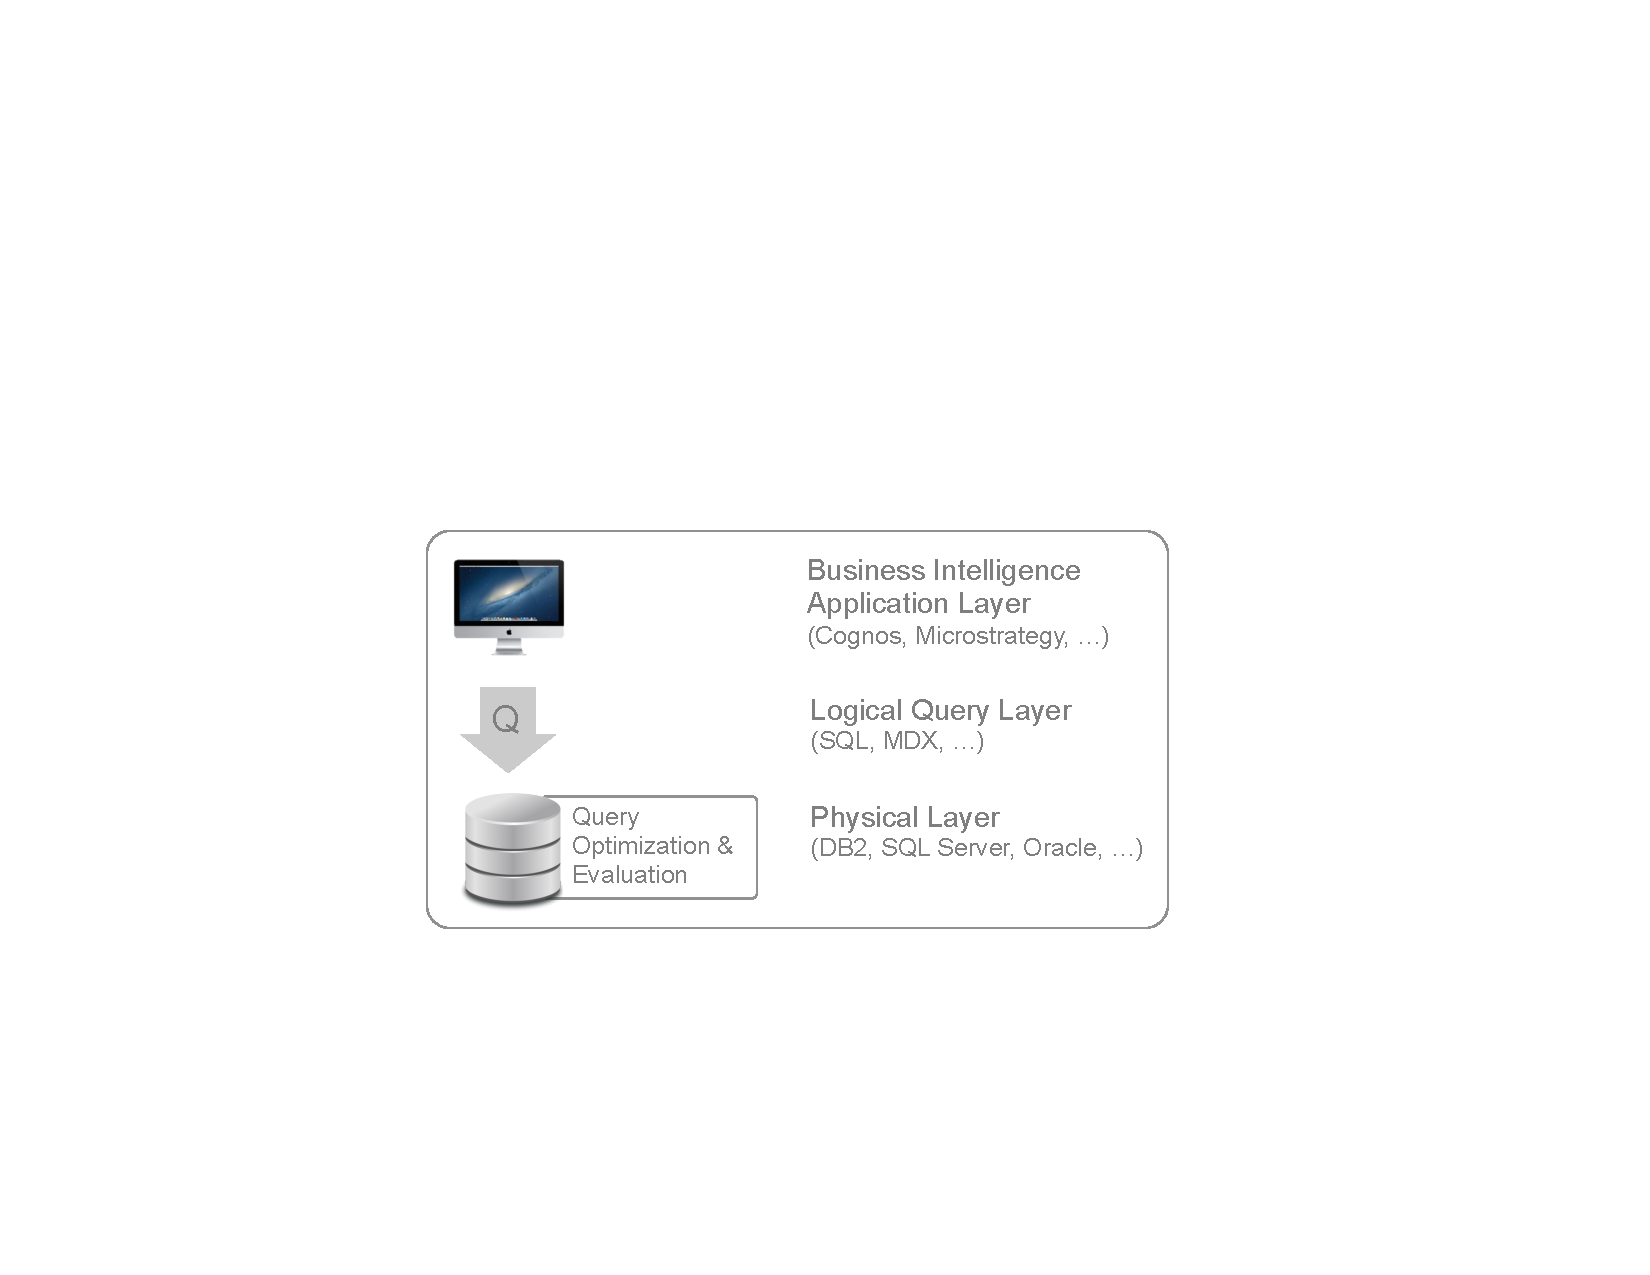
\includegraphics[width=8cm]{fig-dbms.pdf}
\caption{Database-driven analytics architecture}
\label{fig:db-driven-arch}
\vspace*{-0.5cm}
\end{figure}

\subsection{The failure of SQL databases in spatiotemporal sensor data analytics}
\label{sec:the-failure}
In conventional SQL databases, the data contained in the database have a one-to-one mapping to the captured real world objects and events. For example, a database may represent persons, which have an address, a name and a telephone number. Each represented person is supposed to be a corresponding unique entity in the world. Vice versa, as far as the database and the applications running on it are concerned, the represented entities, attributes and relationships constitute the entire real world of interest. In contrast to a conventional database, the sensor data are mere {\em measurements} (samples) of the reality. The full reality of interest to the analytics application is captured by models that predict the quantity of interest at each point in a range of time and/or space. In practice, the gap between the measurements and the real world models is best crossed by learning algorithms that discover the parameters of the real world model and are tuned to the type of the model. For example, when one models a temporal signal exhibiting periodicity, she will use the Fourier transform to discover the frequencies. Given the frequencies, the model can predict a value for any time.

A second cornerstone of statistical sensor data processing, also missed by SQL systems, is the assumption that the real world process that leads to the measurements is a stochastic process. Respectively, an issued query may not return a single predicted value for a quantity; rather, it should return a probability distribution for the predicted value, often simplified by providing an expected value and a confidence interval.

In the absence of real world models in database systems, various suboptimal approaches are used. An approach is to use a database simply as a ``dumb" storage of measurements. Then
given an analytics request, one has to first issue queries that retrieve the relevant measurements. Then she deploys signal processing learning algorithms on them to compute the model's parameters. Finally,  the results are moved into the database. In a variation to this approach, one may not use a SQL database at all (since SQL does not buy her significant functionality anyway) and instead rely on file systems (including the highly scalable distributed file systems). 

In either case, the healthy aspects of SQL database systems discussed in Section~\ref{sec:healthy-aspects} are no longer observed. Instead, the above process is characterized by low productivity as data move in an out of the database in hardwired ways. The approach does not scale to cases with high diversity of data (e.g., when there are ``metadata" and/or other alphanumeric data that provide context to the sensor data analysis and its results) and the analytics application may issue multiple types of  requests. Furthermore, unlike the ecosystem of conventional SQL systems, the analysts of sensor data must be experts of many areas: signal processing, statistics, databases and often big data management and processing. As sensor data proliferate, the short supply of such multiarea experts and the low productivity in developing and maintaining sensor analytics will lead to a world where a lot of sensor data will be collected but only limited analysis will be performed at them, at the cost of missing the insights that these data can offer.

% In a second approach, one may trivialize . For example, This approach can suffer from quality issues and/or performance issues. First, unless the set of measurements is very dense there is a risk that the interpolated values 

In recent years databases have been extended (typically via UDFs) with machine learning procedures that can allow one to execute such procedures without moving data in-and-out of the database. While such extensions are useful, we argue next that they miss the optimization opportunities that become available once models appear in the database as first class citizens and the query language and query processing are adjusted accordingly. Furthermore, they do not account yet for the probabilistic nature of the data and the statistical nature of the queries.

Recent research systems have expanded SQL databases to probabilistic facts (as opposed to the conventional merely boolean facts). As we discuss next, the proposed system assumes that the models are also associated with probabilities.

%The net effect is that analytics on spatiotemporal sensor data currently require the involvement of developers who are essentially skilled in all of the (a) data filtering and combining, (b) modeling, and (c) low level data representation and related algorithms. 
% the decoupling shown earlier has collapsed.

\subsection{Plato: Models as a first class citizen of the database and query language}
\label{sec:plato}
The proposed Plato database has models as a ``first class citizen" abstract type of the database. If we neglect the stochastic aspect of the data, a Plato model is a continuous function over time and/or space that predicts a quantity of interest (eg, temperature, velocity, acceleration, air pollutants density etc) at any coordinate in a certain time/space area. Alternately, a database-minded person may perceive a Plato model as a table whose attributes are time and/or space coordinates and one or more types of quantities. The table has infinitely many tuples and the time/space coordinates form a key, i.e.,  given values for the time/space coordinates, each quantity has a unique associated value. 
In order to capture the stochastic aspect of a process, Plato further assumes that the process may be described by multiple functions, where each function is assigned a probability.

% Queries that one can write.
% Challenge: develop the query languages

Consequently, Plato expands the applicability of the successful architecture of Figure~\ref{fig:db-driven-arch} into statistical, spatiotemporal sensor data management and analytics. The application issues declarative ``Plato SQL" queries, which utilize the models without being concerned about the specifics of how the models are actually represented in the storage nor the intricacies of how to most efficiently execute the queries. (Representation in storage and efficient query execution is introduced next, in Section~\ref{sec:reduced-noise-additive}). \reminder{to YK: place section reference. Check whether these are still the examples we have. I do not mind switching the following to the examples you wrote.} Section~\ref{sec:} provide multiple examples of Plato SQL queries. In one example, a query predicts quantities at specific coordinates; in the stochastic counterpart of the example, the query also asks for the confidence interval, given pi value 0.05. In another example, models are correlated. In a third example, queries drill into specific time segments of the models; e,g., the afternoon times. In yet another example, models capturing the daily paths of individual persons are composed with models that provide the distribution of atmospheric pollutants in San Diego County and the result is models of the pollutant levels that these persons breathed; the query that composes the models is essentially just a simple SQL join. These model-related queries are seamlessly combined with the rest of the database, therefore making it easy to draw results about various segments of the entities represented in the database. For example, a single query can test an hypothesis regarding the inhalation of an atmospheric pollutant by individuals and the asthma attack incidents (as recorded in the conventional medical record) of those individuals.

\subsection{Reduced-noise, additive model representations towards data quality and processing speed}
\label{sec:reduced-noise-additive}
\reminder{Sensor data are unnecessarilly big in their raw form. Yet signal processing research has known for long that data can be split into signal and the often unimportant noise, leading to high effective lossless compression.
}
Obviously, the {\em storage-level representation} (from now on called simply {\em representation}) of the models cannot be the infinitely many possible coordinates and their associated quantities. Fortunately, vast prior work in signal processing research teaches a fruitful connection between good models and high compression. Good models can be represented to high accuracy with much fewer data (model components) than the original measurements data. 
\reminder{to YK, YF: everyone ok with above use of ``model components" for the specific data of the model representation}
Intuitively, the effectiveness of such representations is connected to the physics of the signals. For example, the frequency domain representations generated by Fourier and wavelet transforms capture the periodicity of certain signals. In another example, ARMA models capture the differential equations that govern the connection between neighbor points in time and space.

Plato will be based on a particular variation of models and model representations. The model representation will be {\em additive}, in the sense that the first bits of the representation will provide the most dominant components. Subsequent bits will provide decreasingly important model components. This approach raises the opportunity for a new type of top-k algorithms \cite{Fagin}, which read just enough model components to achieve the level of confidence required by the query.

Eventually, the model representation stops storing additional components when the residual information is white noise. (The project can also expand to other types of noise, e.g., pink noise.) The model components that have been collected up to that point are essentially a more faithful representation of the true underlying real world reality than the original measurements. Practically, this means a data quality advantage: The values predicted by the model are free of the unimportant noise that may have been present in the measurements. These {\em reduced-noise} models are the data quality benefit of a Plato model (and the also the reason for naming the project Plato, in an allusion to Plato's Cave allegory%
\footnote{In Plato's Cave, a few prisoners are bound, since they were born, to look at a wall where shadows of the real world's objects appear. The prisoners perceive only the 2-dimensional world of the shadows and so they miss the deeper insights that a comprehension of the full 3-dimensional reality would offer them. Similarly, the sensor measurements that appear in a database are the mere projection of the real world. The insight in the world is captured by physical models (i.e., models that capture the world's physics). 
}







